\chapter*{Projektphasen, Zeitplanung und Meilensteine}
In den folgenden Abschnitten gehen wir auf die Projektphasen, Zeitplanung und Meilensteine (inkl. Arbeitspakete) ein.

\section*{Projektphasen}
Das Projekt teilt sich in 7 Phasen auf, beginnend mit der Analysephase, und wird mit der Übergabe des Projekts beendet.
\begin{figure}[h]
\centering
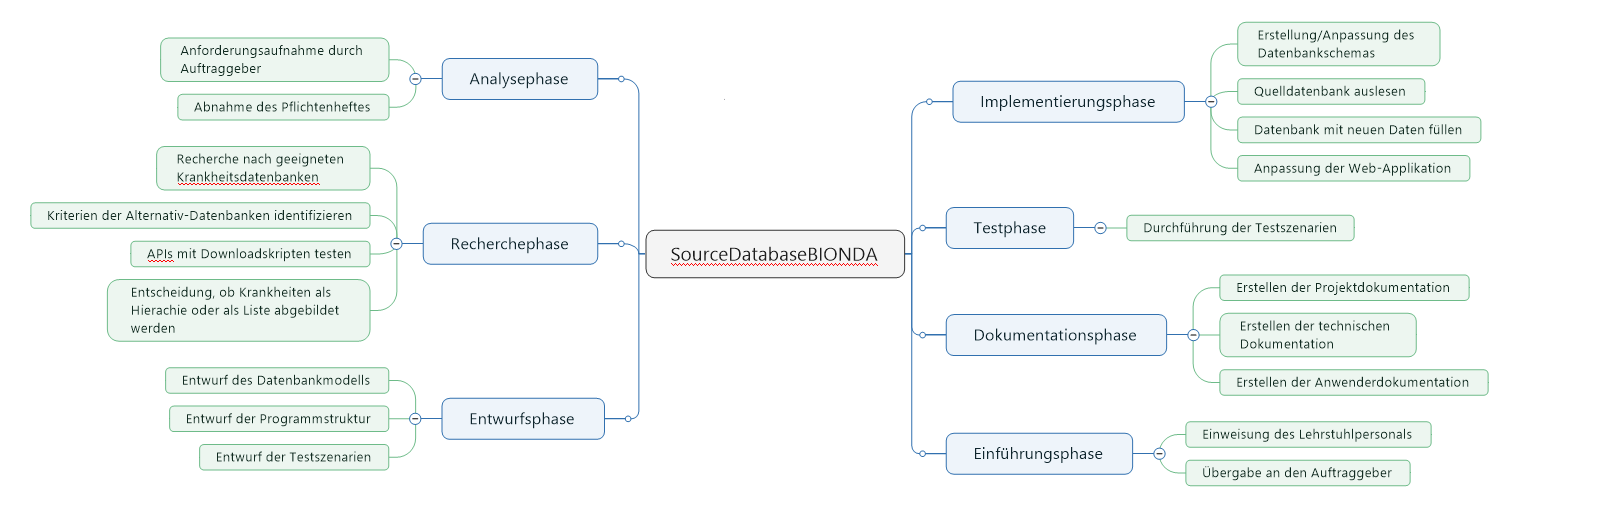
\includegraphics[scale=0.385]{bilder/Projektuebersicht.png}
\caption*{Projektphasen im Überblick}
\end{figure}

\begin{enumerate}
\item Analysephase
\begin{enumerate}[label*=\arabic*.]      
{\item Anforderungsaufnahme durch Auftraggeber} 
{\item Erstellung und Abnahme des Pflichtenheftes} 
\end{enumerate}
\item Recherchephase
\begin{enumerate}[label*=\arabic*.]
{\item Recherche nach geeigneten Krankheitsdatenbanken}       
{\item Kriterien der Alternativ-Datenbanken identifizieren} 
{\item APIs mit Downloadskripten testen} 
{\item Entscheidung, ob Krankheiten als Hierarchie oder als Liste abgebildet werden}
\end{enumerate}
\item Entwurfsphase
\begin{enumerate}[label*=\arabic*.]
{\item Entwurf des Datenbankmodells}       
{\item Entwurf der Programmstruktur} 
{\item Entwurf der Testszenarien} 
\end{enumerate}
\item Implementierungsphase
\begin{enumerate}[label*=\arabic*.]
{\item Erstellung/Anpassung des Datenbankschemas}       
{\item Quelldatenbank auslesen} 
{\item Datenbank mit neuen Daten füllen} 
{\item Anpassung der Web-Applikation}
\end{enumerate}
\item Testphase
\begin{enumerate}[label*=\arabic*.]  
{\item Durchführung der Testszenarien} 
\end{enumerate}
\item Dokumentationsphase
\begin{enumerate}[label*=\arabic*.]
{\item Erstellen der Projektdokumentation}       
{\item Erstellen der technischen Dokumentation}  
{\item Erstellen der Anwenderdokumentation} 
\end{enumerate}
\item Einführungsphase
\begin{enumerate}[label*=\arabic*.]
{\item Einweisung des Lehrstuhlpersonals}       
{\item Übergabe an den Auftraggeber} 
\end{enumerate}
\end{enumerate}

\section*{Arbeitspakete}
Jede Phase des Projekts wurde auch als Arbeitspaket zusammengefasst. Ein Arbeitspaket besteht aus Startdatum und Enddatum, sowie dem Name des Teammitgliedes, das für das Arbeitspaket zuständig ist. 

\subsection*{Analysephase}
\subsubsection*{Arbeitspaket 1.1: Anforderungsaufnahme durch Auftraggeber}
\begin{itemize}
\item Startdatum: 07.10.19
\item Enddatum: 29.10.19
\item Voraussetzung: -
\item Ergebnis: Anforderungen an die Software
\item Verantwortung: Projektteam
\end{itemize}
\subsubsection*{Arbeitspaket 1.2: Erstellung und Abnahme des Pflichtenheftes}
\begin{itemize}
\item Startdatum: 07.10.19
\item Enddatum: 29.10.19
\item Voraussetzung: -
\item Ergebnis: Pflichtenheft
\item Verantwortung: Projektteam
\end{itemize}
\subsection*{Recherchephase}
\subsubsection*{Arbeitspaket 2.1: Recherche nach geeigneten Krankheitsdatenbanken}
\begin{itemize}
\item Startdatum: 19.10.19
\item Enddatum: 25.10.19
\item Voraussetzung: -
\item Ergebnis: Krankheitsdatenbank-Kandidaten liegen vor
\item Verantwortung: Projektteam
\end{itemize}

\subsubsection*{Arbeitspaket 2.2: Kriterien der Alternativ-Datenbanken identifizieren}
\begin{itemize}
\item Startdatum: 19.10.19
\item Enddatum: 25.10.19
\item Voraussetzung: -
\item Ergebnis: Kriterien für den Vergleich liegen vor 
\item Verantwortung: Projektteam
\end{itemize}
\subsubsection*{Arbeitspaket 2.3: APIs mit Download-Skripten testen}
\begin{itemize}
\item Startdatum: 30.10.19
\item Enddatum: 08.11.19
\item Voraussetzung: AP 2.1
\item Ergebnis: Alternativ-DB für BIONDA
\item Verantwortung: Projektteam
\end{itemize}
\subsubsection*{Arbeitspaket 2.4: Entscheidung, ob Krankheiten als Hierarchie oder als Liste abgebildet werden}
\begin{itemize}
\item Startdatum:08.11.19
\item Enddatum: 17.11.19
\item Voraussetzung: AP 2.1, AP 2.3
\item Ergebnis: Plan für die Entwurfsphase
\item Verantwortung: Projektteam
\end{itemize}
\subsection*{Entwurfsphase}
\subsubsection*{Arbeitspaket 3.1: Entwurf des Datenbankmodells}
\begin{itemize}
\item Startdatum: 18.11.19
\item Enddatum: 24.11.19
\item Voraussetzung: AP 2.4
\item Ergebnis: Datenbankmodell
\item Verantwortung: P1
\end{itemize}

\subsubsection*{Arbeitspaket 3.2: Entwurf der Programmstruktur}
\begin{itemize}
\item Startdatum: 18.11.19
\item Enddatum: 24.11.19
\item Voraussetzung: AP 2.4
\item Ergebnis: Programmstruktur
\item Verantwortung: P2
\end{itemize}
\subsubsection*{Arbeitspaket 3.3: Entwurf der Testszenarien}
\begin{itemize}
\item Startdatum: 18.11.19
\item Enddatum: 24.11.19
\item Voraussetzung: AP 2.4
\item Ergebnis: Testszenarien
\item Verantwortung: P3
\end{itemize}
\subsection*{Implementierungsphase}
\subsubsection*{Arbeitspaket 4.1: Erstellung/Anpassung des Datenbankschemas}
\begin{itemize}
\item Startdatum: 25.11.19
\item Enddatum: 09.12.19
\item Voraussetzung: AP 2.1-2.4, AP 3.1-3.3
\item Ergebnis: Angepasstes Datenbankschema
\item Verantwortung: Projektteam
\end{itemize}
\subsubsection*{Arbeitspaket 4.2: Quelldatenbank auslesen}
\begin{itemize}
\item Startdatum: 25.11.19
\item Enddatum: 09.12.19
\item Voraussetzung: AP 2.1-2.4, AP 3.1-3.3
\item Ergebnis: Geparste Dateien
\item Verantwortung: Projektteam
\end{itemize}
\subsubsection*{Arbeitspaket 4.3: Datenbank mit neuen Daten füllen}
\begin{itemize}
\item Startdatum: 09.12.20
\item Enddatum: 19.12.20
\item Voraussetzung: AP 4.1
\item Ergebnis: Integration der Alternativ-Datenbank
\item Verantwortung: Projektteam
\end{itemize}
\subsubsection*{Arbeitspaket 4.4: Anpassung der Web-Applikation}
\begin{itemize}
\item Startdatum: 06.01.20
\item Enddatum: 10.01.20
\item Voraussetzung: AP 4.3
\item Ergebnis: Angepasste Webseite
\item Verantwortung: Projektteam
\end{itemize}
\subsection*{Testphase}
\subsubsection*{Arbeitspaket 5.1: Durchführung der Testszenarien}
\begin{itemize}
\item Startdatum: 11.01.20
\item Enddatum: 11.01.20
\item Voraussetzung: Testszenarien
\item Ergebnis: Es ist bekannt, ob die Software alle Tests erfolgreich durchläuft
\item Verantwortung: Projektteam
\end{itemize}
\subsection*{Dokumentationsphase}
\subsubsection*{Arbeitspaket 6.1: Erstellen der Projektdokumentation}
\begin{itemize}
\item Startdatum: 12.01.20
\item Enddatum: 24.01.20
\item Voraussetzung: fertige Software
\item Ergebnis: Dokumentation über das Projekt
\item Verantwortung: Projektteam
\end{itemize}
\subsubsection*{Arbeitspaket 6.2: Erstellen der technischen Dokumentation}
\begin{itemize}
\item Startdatum: 12.01.20
\item Enddatum: 24.01.20
\item Voraussetzung: fertige Software
\item Ergebnis: Dokumentation über die technischen Hintergründe der Software
\item Verantwortung: Projektteam
\end{itemize}
\subsubsection*{Arbeitspaket 6.3: Erstellen der Anwenderdokumentation}
\begin{itemize}
\item Startdatum: 12.01.20
\item Enddatum: 24.01.20
\item Voraussetzung: fertige Software
\item Ergebnis: Dokumentation für den Anwender
\item Verantwortung: Projektteam
\end{itemize}
\subsubsection*{Arbeitspaket 6.4: Pufferzeit}
\begin{itemize}
\item Startdatum: 24.01.20
\item Enddatum: 31.01.20
\item Voraussetzung: unfertige Arbeitspakete
\item Ergebnis: Vollendung der fehlenden Arbeitspakete 
\item Verantwortung: Projektteam
\end{itemize}
\subsection*{Einführungsphase}
\subsubsection*{Arbeitspaket 7.1: Einweisung des Lehrstuhlpersonals}
\begin{itemize}
\item Startdatum: 02.02.20
\item Enddatum: 02.02.20
\item Voraussetzung: fertige Software
\item Ergebnis: Lehrstuhlpersonal ist in die Software eingewiesen
\item Verantwortung: Projektteam
\end{itemize}
\subsubsection*{Arbeitspaket 7.2: Übergabe an den Auftraggeber}
\begin{itemize}
\item Startdatum: 07.02.20
\item Enddatum: 07.02.20
\item Voraussetzung: fertige Software
\item Ergebnis: Software an den Lehrstuhl übergeben
\item Verantwortung: Projektteam
\end{itemize}

\section*{Meilensteine}
Jede Phase des Projekts endet mit einem Meilenstein. Beim Erreichen des Meilensteins besteht die Möglichkeit die beendete Phase zu überprüfen und einen dieser 3 Wege zu wählen: 

\begin{enumerate}
\item Alle bisherigen Aktivitäten befinden sich im Plan, die Phase kann abgeschlossen werden, das Projekt kann wie geplant fortgesetzt werden.
\item Einige Aktivitäten, die eigentlich laut Planung bereits abgeschlossen sein sollten, weisen in den relevanten Größen (Kosten, Termine, Ergebnisse) signifikante Abweichungen auf. Es muss nachgearbeitet werden, um die Phase abschließen zu können.
\item Es sind Ereignisse eingetreten, die eine sinnvolle Projektfortsetzung unmöglich erscheinen lassen, das Projekt wird gestoppt und ggfs. ganz eingestellt oder unter neuen Rahmenbedingungen völlig neu aufgestellt.
\end{enumerate}

Des Weiteren wird jeder Meilenstein eine Anzahl von Arbeitspaketen zugewiesen. Diese Arbeitspakete sollten zur Deadline des Meilensteins erreicht sein, um eine Verzögerung des Projekts zu vermeiden. Nachfolgend werden die Meilensteine (MS) und Arbeitspakete aufgelistet:

\subsection*{MS 1: Analysephase beendet}
\subsubsection*{Deadline: 29.10.19}
\begin{itemize}
\item Arbeitspaket 1.1: Anforderungsaufnahme durch Auftraggeber
\item Arbeitspaket 1.2: Erstellung und Abnahme des Pflichtenheftes
\end{itemize}

\subsection*{MS 2: Recherchephase beendet}
\subsubsection*{Deadline: 17.11.19}
\begin{itemize}
\item Arbeitspaket 2.1: Recherche nach geeigneten Krankheitsdatenbanken
\item Arbeitspaket 2.2: Kriterien der Alternativ-Datenbank identifizieren
\item Arbeitspaket 2.3: APIs mit Download-Skripten testen
\item Arbeitsoaket 2.4: Entscheidung, ob Krankenheiten als Hierarchie oder Liste abgebildet werden
\end{itemize}

\subsection*{MS 3: Entwurfsphase beendet}
\subsubsection*{Deadline: 24.11.19}
\begin{itemize}
\item Arbeitspaket 3.1: Entwurf des Datenbankmodells
\item Arbeitspaket 3.2: Entwurf der Programmstruktur
\item Arbeitspaket 3.3: Entwurf der Testszenarien
\end{itemize}


\subsection*{MS 4: Implementierungsphase beendet}
\subsubsection*{Deadline: 10.01.20}
\begin{itemize}
\item Arbeitspaket 4.1: Erstellung/Anpassung des Datenbankschemas
\item Arbeitspaket 4.1: Quelldatenbank auslesen
\item Arbeitspaket 4.2: Datenbank mit neuen Daten füllen
\item Arbeitspaket 4.3: Anpassung der Web-Applikation
\end{itemize}

\subsection*{MS 5: Testphase beendet}
\subsubsection*{Deadline: 11.01.20}
\begin{itemize}
\item Arbeitspaket 5.1: Durchführung der Testszenarien
\end{itemize}

\subsection*{MS 6: Dokumentationsphase beendet}
\subsubsection*{Deadline: 24.01.20}
\begin{itemize}
\item Arbeitspaket 6.1: Erstellen der Projektdokumentation
\item Arbeitspaket 6.2: Erstellen der technischen Dokumentation
\item Arbeitspaket 6.3: Erstellen der Anwenderdokumentation
\end{itemize}

\subsection*{MS 7: Pufferzeit ausgeschöpft}
\subsubsection*{Deadline: 31.01.20}
\begin{itemize}
\item Arbeitspaket 6.4: Pufferzeit
\end{itemize}

\subsection*{MS 8: Projekt abgeschlossen}
\subsubsection*{Deadline: 07.02.20}
\begin{itemize}
\item Arbeitspaket 7.1: Einweisung des Lehrstuhlpersonals
\item Arbeitspaket 7.2: Übergabe an den Auftraggeber
\end{itemize}

\begin{figure}[h]
\centering
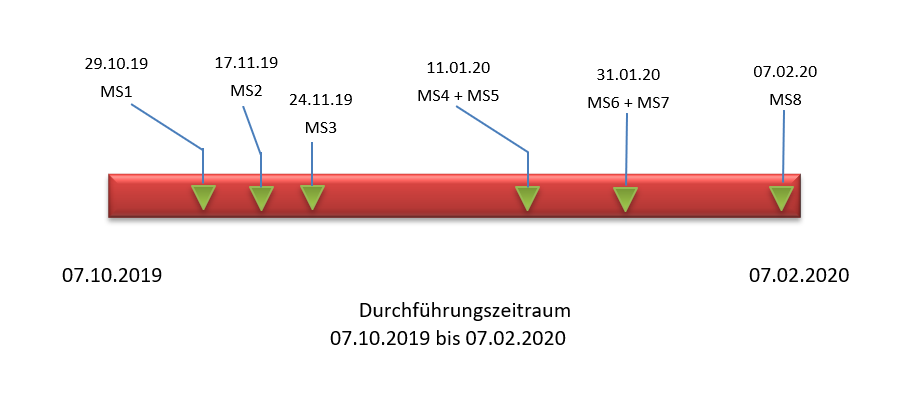
\includegraphics[scale=1]{bilder/Meilensteinplan.png}
\caption*{Meilensteine im Überblick}
\end{figure}